%! Author = user
%! Date = 22.06.2022

% Preamble
\documentclass[11pt]{article}

% Packages
%----------------------------------------------------------------------------------------
%	PACKAGES AND OTHER DOCUMENT CONFIGURATIONS
%----------------------------------------------------------------------------------------

\usepackage{listings}
\usepackage{graphicx}
\usepackage{booktabs}
\usepackage{enumitem}
\usepackage[left=2cm,right=2cm,
    top=2cm,bottom=2cm,bindingoffset=0cm]{geometry}
\usepackage[utf8]{inputenc}
\usepackage[english,russian]{babel}
\usepackage{titling}
\usepackage{textcomp}
\usepackage{mathtext}
\usepackage{amsmath,amsfonts,amssymb,amsthm,mathtools}
\usepackage{icomma}
\usepackage{import}
\usepackage{amssymb, amsmath}
\usepackage{indentfirst}
\usepackage{moresize}
\usepackage{multicol}
\usepackage{dsfont}
\usepackage{xifthen}
\usepackage{pdfpages}
\usepackage{transparent}
\usepackage{caption}
\usepackage{epigraph}
\usepackage{xcolor}

\newtheorem{statement}{Statement}
\newtheorem{corollary}{Corollary}
\newtheorem{theorem}{Theorem}
\newtheorem{definition}{Definition}
\newtheorem{lemma}{Lemma}
\newtheorem{example}{Example}
\theoremstyle{remark}
\newtheorem{remark}{Remark}
\newtheorem{prop}{Property}




\numberwithin{equation}{section} % Number equations within sections (i.e. 1.1, 1.2, 2.1, 2.2 instead of 1, 2, 3, 4)
\numberwithin{figure}{section} % Number figures within sections (i.e. 1.1, 1.2, 2.1, 2.2 instead of 1, 2, 3, 4)
\numberwithin{table}{section} % Number tables within sections (i.e. 1.1, 1.2, 2.1, 2.2 instead of 1, 2, 3, 4)

\setlength\parindent{0pt} % Removes all indentation from paragraphs

\setlist{noitemsep} % No spacing between list items

%%% Операторы всякие:
\DeclareMathOperator{\arsec}{arsec}
\DeclareMathOperator{\arcsch}{arcsch}
\DeclareMathOperator{\arcosh}{arcosh}
\DeclareMathOperator{\arsinh}{arsinh}
\DeclareMathOperator{\artanh}{artanh}
\DeclareMathOperator{\arsech}{arsech}
\DeclareMathOperator{\grad}{grad}
\DeclareMathOperator{\Log}{Log}
\DeclareMathOperator{\Arg}{Arg}
\renewcommand{\Im}{\mathop{\mathrm{Im}}\nolimits}
\renewcommand{\Re}{\mathop{\mathrm{Re}}\nolimits}
\DeclareMathOperator{\arcoth}{arcoth}
\usepackage{setspace}
%%% Колонтитулы
\usepackage{fancyhdr}
\pagestyle{fancy}
\renewcommand{\sectionmark}[1]{\markright{\thesection\ #1}}

\fancyhead[LE,RO]{\thepage}
\fancyhead[LO]{\rightmark}
\fancyhead[RE]{\leftmark}


%----------------------------------------------------------------------------------------
%	SECTION TITLES
%----------------------------------------------------------------------------------------

%\sectionfont{\vspace{6pt}\centering\normalfont\scshape} % \section{} styling
%\subsectionfont{\normalfont\bfseries} % \subsection{} styling
%\subsubsectionfont{\normalfont\itshape} % \subsubsection{} styling
%\paragraphfont{\normalfont\scshape} % \paragraph{} styling

\newcommand{\RNumb}[1]{\uppercase\expandafter{\romannumeral #1\relax}}

\renewcommand\thesection{\arabic{section}.}
\renewcommand\thesubsection{\thesection\arabic{subsection}}
\renewcommand\thesubsubsection{\thesubsection.\arabic{subsubsection}}
\renewcommand{\bf}{\textbf}
%----------------------------------------------------------------------------------------
%	HEADERS AND FOOTERS
%----------------------------------------------------------------------------------------
\DeclareMathOperator{\ord}{ord}
\DeclareMathOperator{\ld}{ld}
\DeclareMathOperator{\exi}{exi}
\DeclareMathOperator{\num}{num}
\DeclareMathOperator{\den}{den}
\DeclareMathOperator{\diam}{diam}
\DeclareMathOperator{\sign}{sign}
\DeclareMathOperator{\len}{len}
\DeclareMathOperator{\vp}{v.p.}
\DeclareMathOperator{\osc}{osc}
\newcommand{\divisible}{\mathop{\raisebox{-2pt}{\vdots}}}
\DeclareRobustCommand{\divby}{%
     \mathrel{\text{\vbox{\baselineskip.65ex\lineskiplimit0pt\hbox{.}\hbox{.}\hbox{.}}}}%
}
\newcommand{\eqdef}{\stackrel{\mathrm{def}}{=}}
\DeclareRobustCommand{\notdivby}{%
     \!\!\not\;\divby%
}
\DeclareMathOperator{\Int}{Int}
\DeclareMathOperator{\Cl}{Cl}
\DeclareMathOperator{\Fr}{Fr}
\newcommand{\Mod}[1]{\ (\mathrm{mod}\ #1)}



\addto{\captionsrussian}{\renewcommand{\abstractname}{АННОТАЦИЯ}}

\newcommand{\incfig}[1]{%
    \def\svgscale{1.5}
    \import{./figures/}{#1.pdf_tex}
}
\graphicspath{{pictures/}}
\DeclareGraphicsExtensions{.pdf,.png,.jpg, .jpeg, .tex}

\definecolor{myblue}{RGB}{72, 184, 178}
\definecolor{myblue1}{RGB}{0, 109, 167}
\usepackage{color}
\usepackage[colorlinks,urlcolor = blue, filecolor=blue,citecolor=blue, linkcolor = blue]{hyperref}

% Document
\begin{document}
    \begin{titlepage}
	\centering
	
	{\Large \textsf{Летняя математическая школа ЛНМО} \par}
	
	\vspace{0.3cm}
	
	{\large \textsf{Поставы, 2022г.}\par}
	
	\vspace{1 cm}
	
	{\HUGE \textsf{Алгебраическая геометрия \\ и теория чисел} \par}
	
	\vspace{0.5cm}
	
	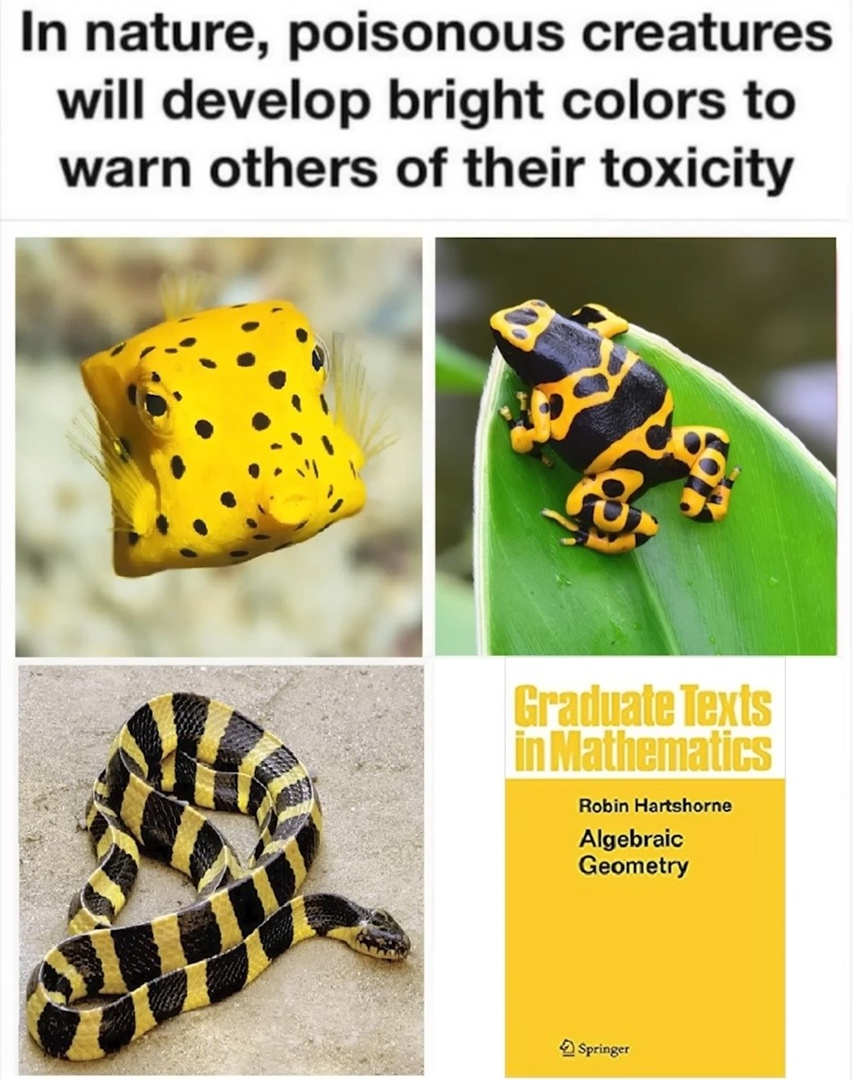
\includegraphics[scale = 0.4]{Title.jpg}
	
	\vspace{0.2cm}
	
	{\large \textsf{\textit{Конспект по материалам лекций, прочитанных М.И. Магиным \\ 11-му математическому классу}} \par}
	\vfill
	
	\begin{minipage}{6in}
		\centering
		\raisebox{-0.5\height}{
\includegraphics[width=0.46\textwidth]{lnmo logo}}
	\end{minipage}


\end{titlepage}

    \begin{center}
        \section*{Алгебраическая геометрия и теория чисел}
    \end{center}
    \tableofcontents
    \newpage

    \section{Нормированные поля}
    \subsection{Нормированное поле. Неархимедовы нормы.}
    Здесь и вдальнейшем будем полагать $F$ полем, хотя многие вещи работают и для кольца (а для области целостности существует
    единственное продолжение на поле частных).

    \begin{definition}\label{fieldnorm}
     Нормой (нормированием, абсолютным значением) на поле $F$  называют отображение $\| \cdot \|\colon F \to \mathbb{R}_{> 0}$,
        удовлетворяющее следующим свойствам:
        \begin{enumerate}
            \item $\| x \| = 0 \Leftrightarrow x = 0$.

            \item $\forall x, y \in F \ \| x y \| = \| x \| \| y \| $.

            \item $\exists C > 0\colon \forall x, y \in F\colon$
            \[ \| x + y \| \le C \cdot \max(\| x \|, \| y \| ) \]
        \end{enumerate}
        Пара $(F, \| \cdot \|)$ называется нормированным полем.
    \end{definition}
    \begin{remark}
        Тем, кто уже до этого видел определение нормы, это определение может показаться странным, так как обычно вместо третьего свойства
        требуют неравенство треугольника:
        \[ \forall x, y \in F \ \| x + y \| \le \| x \| + \| y \| \]
        Ясно, что третье свойство следует из неравенства треугольника с $C = 2$. Ниже мы покажем и обратную импликацию.
    \end{remark}

    Ясно, что любая норма задаёт метрику $d(x, y) = \| x - y \|$, а любая метрика индуцирует топологию стандартным образом.

    \begin{example}
        Если $F \le \mathbb{C}$, то подходит $| \cdot |$ (модуль комплексного числа). Если $F \le \mathbb{R}$ или $F \le \mathbb{Q}$, то подходит $| \cdot |$.
    \end{example}

    \begin{example}
        На любом поле можно ввести тривиальную норму (иногда соответствующую ей метрику называют метрикой лентяя):
        \[ \| x \| = \begin{cases} 0, x = 0 \\ 1, x \neq 0 \end{cases}\]
    \end{example}

    \begin{theorem}
        Если в определении \ref{fieldnorm} постоянная $C$ равна $2$, то норма удовлетворяет неравенству треугольника.
    \end{theorem}
    \begin{proof}

        Сначала отметим, что если $n, m \in \mathbb{N}, \ n \le 2^m$, то в случае произвольной постоянно $C$ выполняется оценка:
        \[ \| x_1 + x_2 + \ldots  + x_n \| \le C^m \cdot \| \max\limits_{1 \le k \le n} \| x_k \| \]
        В самом деле, достаточно просто расписать дерево неравенств. \\
        Отсюда следует неравенство
        \[ \| x_1 + \ldots + x_n \| \le (2n)^{c_0} \max\limits_{1 \le k \le n}(\| x_k \|), \quad c_0 = \log_2{C} \]
        В самом деле, $(2n)^{\log_2{C}} = C \cdot n^{\log_2{C}}$.
        Это также даёт удобную оценку: $\| n \| \le (2n)^{c_0}$.\\
        Теперь заметим, что в нашем случае $c_0 = \log_2{C} = \log_2{2} = 1$, а значит, мы можем провести вот такую
        оценку:
        \begin{multline*} \| x + y \|^n = \| (x + y)^n \| = \left\| \sum\limits_{k = 0}^{n} \binom{n}{k} x^k y^{n - k} \right\| \le 2(n + 1) \max\limits_{0 \le k \le n}\left\| \binom{n}{k} x^k y^{n - k} \right\| \le 2(n + 1) \max\limits_{0 \le k \le n}\left( 2 \binom{n}{k} \|x\|^k \| y \|^{n - k} \right) \le \\
        \le 4(n + 1) (\| x \| + \| y \| )^n \end{multline*}
        Преобразуем это неравенство
        \[ \left( \frac{\| x + y \| }{\| x \| + \| y \|} \right)^n \le 4(n + 1) \leftrightarrow  \frac{\| x + y \|}{\| x \| + \| y \| } \le 4^{\frac{1}{n}} \cdot (n + 1)^{\frac{1}{n}} \]
        В пределе при $n \to \infty$ получаем:
        \[ \frac{\| x + y \| }{\| x \| + \| y \| } \le 1 \Leftrightarrow \| x + y \| \le \| x \| + \| y \| \]
    \end{proof}

    \begin{remark}
        Пример $F = \mathbb{C}$ с нормой $\| \cdot \| = | \cdot |^{\alpha}, \ \alpha > 1$ показывает, что константу $C = 2$ нельзя улучшить.
    \end{remark}
    \begin{remark}
        Тем самым, мы показали, что норму можно понимать, как функтор из категории $\mathcal{F}ield$ в категорию $\mathcal{M}etr$.
    \end{remark}
    \begin{corollary}
        Норма непрерывна.
    \end{corollary}
    \begin{definition}
        Нормы, с постойнной $C = 1$ в определении \ref{fieldnorm} называют неархимедовыми. Нормы, не являющиеся неархимедовыми,
        называют архимедовыми.
    \end{definition}
    \begin{example}
        Тривиальная норма на любом поле $F$ является неархимедовой.
    \end{example}
    \begin{definition}
        Ясно, что любое $x \in \mathbb{Q}$ представимо в виде $x = p^n \cdot \frac{a}{b}$, где $a, b \in \mathbb{Z}, \ a \not\divisible p, \ a \not\divisible p$, а $n \in \mathbb{Z}$.
        В таком случае число $n$ называют $p$-адическим показателем числа $x$ и обозначают $\upsilon_p(x)$.
    \end{definition}
    \begin{definition} \textbf{(Самое важное)}\\
    Пусть $p$~--- простое число. Тогда норму
        \[ \| x \|_{p} = \begin{cases} 0, x = 0 \\ p^{-\upsilon_p(x)}, x \neq 0  \end{cases}\]
    на поле $\mathbb{Q}$ называют $p$-адической нормой.
    \end{definition}

    \begin{remark}
        Ясно, что подоходит $r^{-\upsilon_p(x)}$, где $r > 1$, но $p$ брать удобно, так как для $x \in \mathbb{Q}^{*}$ справедлива формула произведения
        \[ 1 = \prod\limits_{p} |x| \cdot  \| x \|_{p} \]
    \end{remark}
    \begin{lemma}
        Если норма неархимедова, то для $x, y\colon \| x \| \neq \| y \|$ выполняется $\| x + y \| = \max{\| x \|, \| y \| }$.
    \end{lemma}
    \begin{corollary}
        Рассмотрим $(F, \| \cdot \| )$, где норма $\| \cdot \|$ неархимедова. Тогда, если  $b \in B_r(a)$, то $B_r(a) = B_r(b)$.
     \end{corollary}
    \begin{corollary} (Забавное)\\
        Если на поле $F$ введена неархимедова норма $F$, то $\forall x, y, z \in F$ по крайней мере два числа из
        $\| x - y \|, \ \| x - z \|, \ \| y - z\| $ равны. \\
        Иными словами, в метрическом пространстве $(F, d)$ ($d(x, y) = \| x - y \| $) все треугольники равнобедренные.
    \end{corollary}

   \section{$p$-адические числа}
   \subsection{Кольцо целых $p$-адических чисел.}

    Прежде чем давать какие-либо определения, рассмотрим следующий мотивирующий пример. \\
    Рассмотрим сравнение $x^2 \equiv 2 \pmod{7^n}$, $n \in \mathbb{N}$. Если $n = 1$, то ясно, что
    \[ x_0 \equiv \pm 3 \pmod{7} \]
    Теперь рассмотрим $n = 2$. $x^2 \equiv 2 \pmod{7^2} \Rightarrow x^2 \equiv 2
    \pmod{7}$, а значит, рещения сравнения с $n = 2$ надо искать в виде $x_0 + 7t_1$.\\
    Займемся поиском решений вида $x_1 = 3 + 7t_1$. Подставим:
    \[ (3 + 7t_1)^2 \equiv 2 \pmod{7^2} \Leftrightarrow 9 + 6 \cdot 7t_1 + 7^2 t_1^2 \equiv 2 \pmod{7^2} \Rightarrow 1 + 6t_1 \equiv 0 \pmod{7} \Rightarrow t_1 \equiv 1 \pmod 7 \]
    Отсюда имеем решение  $x_1 \equiv 3 + 7 \cdot 1 \pmod{7^2}$.\\
    При $n = 3$ мы получим $x_2 = x_1 + 7^2 t_2$ и подставляя
    \[ (3 + 7 + 7^2 t_2)^2 \equiv 2 \pmod{7^3} \]
    мы найдём $t_2 \equiv 2 \pmod{7}$, а значит,
    \[ x_2 \equiv 3 + 7 \cdot 1 + 7^2 \cdot 2 \pmod{7^3} \]
    Продолжая этот процесс, получим последовательность $x_0, x_1, x_2, \ldots, x_n, \ldots$ со свойствами
    \[ x_0 \equiv 3 \pmod{7}, \quad x_n \equiv x_{n - 1} \pmod{7^n}, \quad x_n^2 \equiv \pmod{7^{n + 1}} \]

    Процесс построения этой последовательности может напонмить внимательному читателю процесс вычисления $\sqrt{2}$
    при помощи приблиэения рациональными числами. Там мы тоже строим последовательность рационаьных чисел
    $r_1, r_2, \ldots, r_n$, квадраты которых становятся сколь угодно близки к 2, например, $|r_n^2 - 2|< 1/10^n$.

    Если мы зафиксируем простое число $p$ будем считать два целых числа близкими, если их разность делится на достаточно большую
    степени $p$ (то есть, близкими в смысле $p$-адической метрики):
    \[ d_p(x, y) = \| x - y \|_p = p^{-\upsilon_p(x - y)}\]
    В конкретном примере выше,
    \[ \forall \varepsilon > 0 \ \exists N\colon \forall n \ge N \  d_7(x_n^2, 2) < \varepsilon \]
    Как мы помним, задание последовательности рациональных чисел $\{ r_n \}$ определяет вещественное число $\sqrt{2}$.
    Проводя аналогию, здесь мы также можем предположить, что последовательность $\{ x_n \}$ определяет некоторое
    число $\alpha$ совершенно новой природы. \\
    Заметим также, что если у нас есть такая последовательность рациональных чисел $\{ r'_n \}$, что $\forall \varepsilon > 0 \ \eists N\colon \forall n > N \ |r_n - r'_n| < \varepsilon $, то
    её пределом также будет $\sqrt{2}$ (и в этом смысле определение корректно).\\
    Соответсвенно, здесь нам также будет естественно предположить, что последовательность $\{ x'_n \}$, для которой $x_n \equiv x'_n \pmod{7^{n + 1}}$  определяет то же самое число $\alpha$.
    \begin{remark}
        В общем, во всей этой аналогии мы просто заменили метрику на $p$-адическую.
    \end{remark}
    \begin{definition}
        Пусть $p$~--- некоторое простое число. Последовательность целых чисел $\{ x_n \}$, обладающих свойством
        \[ x_n \equiv x_{n - 1} \pmod{p^n} \ \forall n \ge 1\]
        определяет новый объект, называемый $p$-адическим числом. Две последовательности $\{ x_n \}$ и $\{ x'_n \}$ определяют одно и то же
        целое $p$-адическое число, когда $x_n \equiv x'_n \pmod{p^{n + 1}} \ \forall n \ge 0$.\\
        То есть, целые $p$-адические числа~--- предел по $p$-адическое норме целых.\\
        Множество всех целых $p$-адических чисел мы будем обозначать через $\mathbb{Z}_p$.\\
    \end{definition}
    Обычные целые числа (не $p$-адические) будем с этого момента называть целыми рациональными.\\


    Заметим, что каждому целому рациональному числу $x$ можно сопоставить целое $p$-адиеческое число, определяемое последовательностью
    $\{ x, x, x, \ldots \}$. Такое целое $p$-адическое число мы будем обозачать той же буквой $x$. Таким образом, мы получили естественное
    вложение $\mathbb{Z} \hookrightarrow \mathbb{Z}_p$ (инективность вполне очевидна).

    \begin{remark} \textbf{Канонический способ задания $p$-адического числа.}\\
        Пусть целое $p$-адическое число задается последовательностью $\{ x_n \}$. Обозначим наименьшее неотрицательное
        число, сравнимое с $x_n$ по модулю $p^{n + 1}$ за $\overline{x_n}$.
        \[ x_n \equiv \overline{x_n} \pmod{p^{n + 1}}, \ 0 \le \overline{x_n} < p^{n + 1} \]
        Ясно, что
        \[ \overline{x_n} \equiv x_n \equiv x_{n - 1} \equiv \overline{x_{n - 1}} \pmod{p^n}\]
        То есть, последовательность $\{ \overline{x_n} \}$ определяют то же целое $p$-адическое число, что и $\{ x_n \}$.
        Заметим, что если две последовательности $\{ \overline{x_n} \}$ и $\overline{y_n}$ определяют одно и то же целое $p$-адическое число, то
        в силу
        \[ \overline{x_n} \equiv \overline{y_n} \pmod{p^{n + 1}}, \ 0 \le \overline{x_n} < p^{n + 1}, \ 0 \le \overline{y_n} < p^{n + 1}\]
        мы имеем $\overline{x_n} = \overline{y_n}$, то есть, такое представление единственно. Его мы и будем называть каноническим представлением. \\


        Заметим, что $\overline{x^n} \equiv \overline{x_{n - 1}} \pmod{p^n}$, а так как $0 \le \overline{x_n} < p^{n + 1}$, вся каноническая
        последовательность имеет вид
        \[ \{ a_0, \ a_0 + a_1 p, \ a_0 + a_1 p + a_2 p^2, \ldots \}, \quad 0 \le a_i < p \]
        С другой стороны, ясно, что каждая последовательность такого вида задаёт некоторое целое $p$-адическое число.
    \end{remark}

    Ясно, что операции сложения и умножения на $p$-адических числах определяются поточечными операциями с соответствующими
    последовательностями.

    Все свойства операций очевидны, значит, $\mathbb{Z}_p$~--- коммутативное кольцо. Поймём что-нибудь про множество обратимых элементов кольца.

    \begin{theorem}
        Целое $p$-адическое число $\alpha$, определяемое
        последовательностью $\{ x_0, x_1, \ldots, x_n, \ldots \}$ я тогда и только тогда, когда $x_0 \not\equiv 0 \pmod{p}$.
    \end{theorem}
    \begin{proof}
        Путь $\alpha \in \mathbb{Z}_p^{*}$. Тогда существует такое целое $p$-адическое число $\beta$, что $\alpha \beta = 1$. \\
        Пусть $\beta$ определяется последовательностью $\{ y_n \}$. Тогда
        \[ x_n y_n \equiv 1 \pmod{p^{n + 1}} \]
        В частности, $x_0 y_0 \equiv 1 \pmod{p} \Rightarrow x_0 \not\equiv 0 \pmod{p}$. И обратно, так как $x_0 \not\equiv 0 \pmod{p}$ и $x_n \equiv x_{n - 1} \pmod{p^n}$ мы имеем
        \[ x_n \equiv x_{n - 1} \equiv \ldots \equiv x_0 \pmod{p} \Rightarrow x_n \not\equiv 0 \pmod{p} \]
        Значит, так как $p$~--- простое, $\forall n \ \exists y_n \colon x_n y_n \equiv 1 \pmod{p^{n + 1}}$.
        \[ x_n \equiv x_{n - 1} \pmod{p^n}, \ x_n y_n \equiv x_{n - 1} y_{n - 1} \pmod{p^n} \Rightarrow y_n \equiv y_{n - 1} \pmod{p^n} \]
        а значит, $\{ y_n \}$ определяет некоторое целое $p$-адическое число $\beta$.\\
        Таким образом, $\alpha \beta = 1 \Rightarrow \alpha \in \mathbb{Z}_p^{*}$.
    \end{proof}

    \begin{theorem}\label{predstp-adic}
        Любое отлчиное от нуля целое $p$-адическое число $\alpha$ можно единственным образом представить в виде
        \[ \alpha = p^m \cdot \varepsilon, \quad \varepsilon \in \mathbb{Z}_p^{*}, \ m \in \mathbb{N} \]

    \end{theorem}
    \begin{proof}
        Если $\alpha \in \mathbb{Z}_p^{*}$, то равенство справедливо при $m = 0$.\\
        Пусть теперь $\alpha \notin \mathbb{Z}_p^{*}$ и $\{ x_n \} \to \alpha$. Тогда, по предыдущей теореме
        $x_0 \equiv 0 \pmod{p}$. Так как $\alpha \neq 0, \ \exists N \in \mathbb{N}\colon \forall n \ge N \ x_n \not\equiv 0 \pmod{p^{n + 1}}$.
        Пусть $m$~--- наимеьший индекс, для которого
        \[ x_m \not\equiv 0 \pmod{p^{m + 1}}\]
        Заметим, что в таком случае $\forall s \ge 0$
        \[ x_{m + s} \equiv x_{m - 1} \equiv 0 \pmod{p^{m}} \Rightarrow y_s = \frac{x_{m + s}}{p^m} \in \mathbb{Z} \]
        \[ p^m y_s - p^m y_{s - 1}  = x_{m + s} - x_{m + s - 1} \equiv 0 \pmod{p^{m + s}} \Rightarrow y_s \equiv y_{s - 1} \pmod{p^s}\]
        То есть, последовательность $\{ y_s \}$ тоже определяет некоторое $p$-адическое число $\varepsilon \in \mathbb{Z}_p$.
        Заметим, что $y_0 = x_m/p^m \not\equiv 0 \pmod{p} \Rightarrow \varepsilon \in \mathbb{Z}_p^{*}$.\\
        Из сравнения
        \[ p^m y_s = x_{m + s} \equiv x_s \pmod{p^{s + 1}} \]
        следует, что $\alpha = p^m \cdot \varepsilon$.
        Покажем теперь единственность. Предположим, что $\alpha = p^k \xi, \ k \ge 0, \ \xi \in \mathbb{Z}_{p}^{*}$. Пусть $\{ z_s \} \to \xi$.
        \[ p^m y_s \equiv p^k z_s \pmod{p^{s + 1}} \ \forall s \ge 0 \]
        Так как $\varepsilon$ и $\xi$~--- обратимые элементы кольца, по предыдущей теореме $y_s \not\equiv 0 \pmod{p}, \ z_s \not\equiv 0 \pmod{p}$.
        Подставим в предыдущее сравнения $s = m$:
        \[ p^m y_m \equiv p^k z_m \not\equiv 0 \pmod{p^{m + 1}} \Rightarrow k \le m \]
        Так как мы можем проделать то же самое абсолютно симметрично для $k$, мы также имеем $k \ge m$, а значит
        $k = m$.
        То есть, мы получили, что $y_{m + s} \equiv z_{m + s} \pmod{p^{s + 1}}$, а так как $y_{s + 1} \equiv y_s \pmod{p^{s + 1}}, \ z_{s + 1} \equiv z_s \pmod{p^{s + 1}}$,
        мы имеем $z_s \equiv y_s \pmod{p^{s + 1}} \ \forall s \ge 0 \Rightarrow \varepsilon = \xi$.
    \end{proof}
    \begin{corollary}
        $\mathbb{Z}_p$~--- область целостности.
     \end{corollary}
    \begin{proof}
        Упражнение в листочке.
    \end{proof}

    Теперь ясно, что число $m$ в представлении $\alpha = p^m \varepsilon$~--- $p$-адический показатель $\alpha$ ($\upsilon_p(\alpha)$).

    В терминах $p$-адического показателя легко вырадать свойства делимости $p$-адических чисел.
    \begin{corollary}
        Целое $p$-адическое число $\alpha$ делится на целое $p$-адическое число $\beta$ тогда и только тогда, когда
        $\upsilon_p(\alpha) \ge \upsilon(\beta)$.
     \end{corollary}

    Резюмируя всё это, мы получили, что в кольце $\mathbb{Z}_p$ всего один (с точностью до ассоциированности) простой элемент~--- число $p$,
    а все остальные (отличные от нуля)~--- его степени, домноженные на обратимые.
    \subsection{Локализация и поле частных колцьа.}

    Вообще, эта тема совершенно никак не относится к программе курса, но, прочитать всё равно надо.

    \textcolor{blue}{Идея:} уметь обращать набор элементов кольца \emph{универсальным} образом. \\

    \begin{remark}
        Отметим, что обратимый элемент не может являться делителем нуля, поэтому, если мы хотим обращать делители нуля,
        все элементы, которые в произведении с ним дают 0 должны перейти в 0. Кроме того, если два элемента обратимы, то их
        произведение обратимо. Кроме того, если мы добавим в множество, которое хотим обращать единицу, то ничего не изменится, так как
        умножение на единицу ничего не меняет. \\

        Таким образом, будем заниматься обращением множеств, замкнуты относительно умножения и содержат единицу (будем называть такие
        множества мультипликативными).
    \end{remark}
    \textcolor{blue}{Тут можно рассказать, с чего бы это называется локализацией, но как-то лень, если время останется, расскажу.}
    \begin{definition}
        Пусть $S$~--- мультипликативное подмножество кольца $R$. Локализацией кольца $R$ в $S$ называется кольцо $S^{-1}R$ вместе с
        локализационным гомоморфизмом $\lambda_s\colon R \to S^{-1}R$, удовлетворяющее свойствам
        \begin{enumerate}
            \item $\forall s \in S \ \lambda_s(s)$ обратим в $S^{-1}R$.
            \item Для любого гомоморфизма $\varphi\colon R \to A$, при котором $\varphi(s) \in A^{*}$ для всех $S$ существует
                  единственный гомоморфизм $\psi\colon S^{-1}R \to A$ такой, что $\psi \circ \lambda_s = \varphi$.
                  Иными словами, коммутативна диаграмма
                  \begin{center}
                      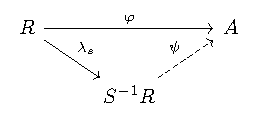
\includegraphics[scale = 1]{cd.pdf}
                  \end{center}

        \end{enumerate}
    \end{definition}

    Как и всегда, определение объекта через универсальное свойство ничего не говорит о существовании объекта, поэтому
    сейчас мы будем больно и мучительно строить локализацию.\\

    \textbf{Построение локализации:}\\

    Определим отношение $\sim$ на множестве $R \times S$ по правилу
    \[ (r_1, s_1) \sim (r_2, s_2) \Longleftrightarrow s s_2 r_1 = s s_1 r_2 \]
    \begin{remark}
        Здесь мы домножаем на $s$ как раз за тем, чтоб делители нуля ушли в ноль.
    \end{remark}
    \begin{statement}
        $\sim$~--- отношение эквивалентности.
    \end{statement}
    \begin{proof}
        Рефлексивность и симметричность очевидны. \\
        Самое неприятное~--- транзитивность.\\
        Пусть $(r_1, s_1) \sim (r_2, s_2)$ и $(r_2, s_2) \sim (r_3, s_3)$, то есть
        \[ s r_1 s_2 = s r_2 s_1, \quad s' r_2 s_3 = s' r_3 s_2, \ s, s' \in S \]
        Домножим первое равенство $s' s_3$, а второе $s s_1$, получим
        \[ s r_1 s_2 = s r_2 s_1 \to s' s_3 s r_1 s_2 = \textcolor{blue}{s' s_3 s r_2 s_1}, \qquad s' r_2 s_3 = s' r_3 s_2 \to \textcolor{blue}{s s_1 s' r_2 s_3}  = s s_1 s' r_3 s_2 \]
        Остается заметить, что
        \[ s s' s_2 \in S \Rightarrow (r_1, s_1) \sim (r_3, s_3) \]
        то есть, транзитивность доказана.
    \end{proof}

    Теперь, положим $S^{-1}R = R \times S / \sim$. Класс эквивалентности, содержащий представитель $(r, s)$ будем обозначать
    $\frac{r}{s}$.\\
    Определим локализационный гомоморфизм $\lambda_s\colon R \to S^{-1}R$ формулой $\lambda_{S}(r) = \frac{r}{1}$.\\

    \textcolor{blue}{Теперь, научимся складывать дроби.}

    \begin{theorem}
        Пусть $S$~--- мультипликативное подмножество кольца $R$. Определим на $S^{-1}R$ операции следующим образом
        \[ \frac{r_1}{s_1} \cdot \frac{r_2}{s_2} = \frac{r_1 r_2}{s_2 s_2}, \quad \frac{r_1}{s_1} + \frac{r_2}{s_2} = \frac{s_1 r_2 + s_2 r_1}{s_1 s_2} \]
        Тогда $S^{-1}R$~--- локализация $R$ в мультипликативном подмножестве $S$ с локализицонном гомоморфизмом $\lambda_s$ (как написано выше).
    \end{theorem}
    \begin{proof}
        Докажем сначала, что наше определение сложения и умножения не зависит от выбора представителя. \\
        Пусть выплняются равенства
        \[ \frac{r_1'}{s_1'} = \frac{r_1}{s_1} \leftrightarrow s r_1 s_1' = s r_1' s_1, \quad \frac{r_2'}{s_2'} = \frac{r_2}{s_2} \leftrightarrow s' r_2 s_2' = s' r_2' s_2 \]
        Перемножим последние равенства
        \[ s s' r_1 s_1' r_2 s_2' = s s' r_1' s_1 r_2' s_2 \]
        Отсюда имеем
        \[ \frac{r_1 r_2}{s_1 s_2} = \frac{r_1' r_2'}{s_1' s_2'} \]
        Далее, будет некоторая \textcolor{red}{боль}, а именно, надо доказать
        \[ \frac{r_1 s_2 + r_2 s_1}{s_1 s_2} = \frac{r_1' s_2' + r_2' s_1' }{s_1' s_2'} \]
        Если Вы немного помедитируете на формулы ниже, станет понятно, почему это так:
        \[ ss' (r_1 s_2 + r_2 s_1) s_1' s_2' = s s' (e_1 s_2 s_1' s_2' + r_2 s_1 s_1' s_2') =
        s s' (r_1' s_2 s_1 s_2' + r_2' s_1 s_2' s_2) = s s' (r_1' s_2' + r_2' s_1') s_1 s_2 \]
        Вообще, честно говоря, также нужно доказывать ассоциативность сложения, коммутативность и дистрибутивность.
        Давайте непосредственно проврим ассоциативность сложения
        \[ \left( \frac{r_1}{s_1} + \frac{r_2}{s_2} \right) + \frac{r_3}{s_3} = \frac{r_1 s_2 + r_2 s_1}{s_1 s_2} + \frac{r_3}{s_3} = \frac{r_1 s_2 s_3 + r_2 s_1 s_3 + r_3 s_1 s_2}{s_1 s_2 s_3} \]
        \[ \frac{r_1}{s_1} + \left( \frac{r_2}{s_2} + \frac{r_3}{s_3} \right) = \frac{r_1}{s_1} + \frac{r_2 s_3 + r_3 s_2}{s_2 s_3} = \frac{r_1 s_2 s_3 + r_2 s_3 s_1 + r_3 s_2 s_1}{s_1 s_2 s_3}\]
        Нейтральным элементом по сложению будет $\frac{0}{1} = \frac{0}{s}$, обратным по сложению к $\frac{r}{s}$~--- $-\frac{r}{s}$.
        Нейтральным элементом по умножению~---$\frac{1}{1} = \frac{s}{s}$. Проверим свочтва локализации:
        \[ \lambda_s(s) \cdot \frac{1}{s} = \frac{s}{1} \cdot \frac{1}{s} = 1 \]
        то есть, первое свойство выполнено. \\

        Пусть $\varphi\colon R \to A$~--- такой гомоморфизм колец, что $\varphi(s) \in A^* \ \forall s \in S$.
        Определим отображение $\psi\colon S^{-1}R \to A$ равенством $\psi(\frac{r}{s}) = \varphi(r) \varphi(s)^{-1}$. \\

        Если $\frac{r'}{s'} = \frac{r}{s}$, то по определению
        \[ \frac{r'}{s'} = \frac{r}{s} \Leftrightarrow r' s = r s', \ s'' \in S \Rightarrow \varphi(s'')\varphi(r')\varphi(s) = \varphi(s'') \varphi(r) \varphi(s') \]
        Домножим на $\varphi(s'')^{-1} \varphi(s')^{-1} \varphi(s')^{-1}$, получим
        \[ \varphi(r') \varphi(s')^{-1} = \varphi(r) \varphi(s)^{-1} \]
        а значит, $\psi$ определён корректно. Так как $\varphi(1) = 1$, имеем $\varphi = \psi \circ \lambda_{S}$. Ясно, что $\psi$~--- гомоморфизм. \\

        Равенство $\varphi = \psi \circ \lambda_{S}$ однозначно задаёт $\psi(\frac{r}{1}) = \varphi(r)$. Так как $\psi$ должен
        быть гомоморфизмом,
        \[ \varphi(r) = \psi(\frac{r}{1}) = \psi(\frac{r}{s} \cdot \frac{s}{1}) = \psi(\frac{r}{s}) \cdot \varphi(s) \]
        Так как по условию $\varphi(s) \in A^*$, имеем $\psi(\frac{r}{s}) = \varphi(r)\varphi(s)^{-1}$, что завершает доказательство.


    \end{proof}

    \textsc{\textbf{Примеры локализации:}}
    \begin{enumerate}
        \item Для $s \in R$ положим $\langle s \rangle = \{ s^n \ | \ n \in \mathbb{N} \}$. Локализация $\langle s \rangle^{-1}R$
              обозначается через $R_s$ и называется главной локализацией в элементе $s$ (по аналогии с главным идеалом).
        \item Если $P$~--- простой идеал кольца $R$, то $R \setminus P$ является мультипликативным подмножеством.
              В этом случае локализация $R_{P} = (R \setminus P)^{-1} R$ называется локализацией $R$ в простом идеале $P$.
              $R_P$ является локальным кольцом (т.е. кольцом с единственным максимальным идеалом).
        \item $S$~--- множество всех элементов $R$, не являющийся делителями нуля. Тогда $S^{-1}R$ называется полным кольцом частных
              кольца $R$. Это максимальная локализация, для которой гомоморфизм локализации инъективен.
    \end{enumerate}

    Если $R$~--- область целостности, то $\{ 0 \}$~--- простой идеал. Локализация в этом идеале, очевидно,
    будет полем, которое называется полем частных кольца $R$.\\

    Иными словами, поле частных~--- это полное кольцо частных области целостности. Локализационный гомоморфизм~--- это
    универсальное вложение в следующем смысле:

    \begin{lemma}
        Пусть $R$~--- область целостности, а $S = R\seminus \{ 0 \}$. Тогда $F = S^{-1}R$ является полем, а гомоморфизм
        локализации $\lambda_{S}\colon R \to F$ инъективен, а $\lambda_{S}$ удовлетворяет следующему универсальному свойству:
        для любого поля $K$ и мономорфизма $R \to K$ существует единственный мономорфизм $\psi\colon F \to K$, что $\varphi = \psi \circ \lambda_s$.
    \end{lemma}

    \subsection{Поле $p$-адических чисел, как поле частных кольца $\mathbb{Z}_p$.}

    Как мы уже выяснили, кольцо $\mathbb{Z}_p$~--- область целостности, его можно вложить в поле частных, используя
    конструкцию локализации.\\
    В нашем случае это сводится к рассмотрению дробей $\alpha / p^k$, где $\alpha \in \mathbb{Z}_p, \ k \ge 0$.
    \begin{definition}
        Дробь вида $\alpha / p^k$, где $\alpha \in \mathbb{Z}_p$, а $k \ge 0$ называется дробным $p$-адмическим числом
        или просто $p$-адическим числом.
    \end{definition}
    \begin{remark}
         Две дроби $\alpha / p^k$ и $\beta / p^m$ определяют одно и то же $p$-адическое число, если $\alpha p^m = \beta p^k$.
    \end{remark}

    \begin{definition}
        Полем  $p$-адических чисел $\mathbb{Q}_p$ называется поле частных кольца целых $p$-адических чисел $\mathbb{Z}_p$.
    \end{definition}

    \begin{theorem}
        Всякое $p$-адическое число $\xi \neq 0$ единственным образом представляется в виде
        \[ \xi = p^m \cdot \varepsilon, \quad m \in \mathbb{Z}, \ \varepsilon \in \mathbb{Z}_p^{*} \]
    \end{theorem}
    \begin{proof}
        Пусть $\xi = \alpha / p^k, \ \alpha \in \mathbb{Z}_p$. По теореме \ref{predstp-adic}  $\alpha$ можно представить в виде
        $p^{\ell} \varepsilon, \ \ell \ge 0, \varepsilon \in \mathbb{Z}_p^{*}$. Тогда $\xi = p^m \varepsilon, m = \ell - k$.\\
        Единственность вытеакет из единственности представления для \ref{predstp-adic}.
    \end{proof}

    \subsection{Сходимость в поле $p$-адических чисел}
    Мы уже много раз говорили об аналогии между $p$-адическими числами и вещественными. В случае вещественных, они определяются последовательностями
    рациональных и являются пределами этих последоватлеьностей. \\

    Неформально мы уже обсуждали, почему это так в случае $p$-адических чисел, давайте теперь поймем, почему это так формально. \\

    Теперь, после того как мы доопределили $p$-адический показатель на $\mathbb{Q}_p$, мы можем вводить на $\mathbb{Q}_p$ (заметьте, уже не на $\mathbb{Q}$) знакомое
    нам  $p$-адическое нормирование (и, соответственно, $p$-адическую метрику).

    \begin{definition}
        Последовательность $p$-адических чисел $\{ \xi_n \}$ называется сходящейся к $p$-адическому числу  $\xi$ если
        \[ \lim\limits_{n \to \infty} \upsilon_p(\xi_n - \xi) = \infty \]
    \end{definition}
    \begin{remark}
        Ясно, что эквивалентно сходимость можно определять, как
        \[ \lim\limits_{n \to \infty} \{ \xi_n \} = \xi \Leftrightarrow \lim\limits_{n \to \infty}\| \xi_n - \xi \| = 0\]
        то есть, как и обычно, начиная с некоторого довольно большого номера, $p$-адические числа становятся сколь угодно близки к пределу.
    \end{remark}
    Рассмотрим сначала для удобства некоторые свойства $p$-адического показателя:
    \begin{enumerate}
        \item $\upsilon_{p}(\alpha \beta) = \upsilon_p(\alpha) + \upsilon_p{(\beta)} $.

        \item $ \upsilon_p{(\alpha + \beta)} \ge \min(\upsilon_p{(\alpha)}, \upsilon_p{(\beta)})$.

        \item $ \upsilon_p{(\alpha + \beta)} = \min{( \upsilon_p{(\alpha)}, \upsilon_p{(\beta)})}, \ \alpha \neq \beta$.
    \end{enumerate}
    Для поля $\mathbb{Q}_p$ справедливы все стандартные свойства пределов. Докажем, например, что при $\{ \xi_n \} \to \xi, \ \xi \in \mathbb{Z}_p^{*}$ выполняется $\{ 1 / \xi_n \} \to 1 / \xi_n$. \\

    Сначала отметим, что, начиная с некоторого места $ \upsilon_p{(\xi_n - \xi)} > \upsilon_p{(\xi)}$, откуда $ \upsilon_p{(\xi_n)} = \min( \upsilon_p{(\xi_n - \xi)}, \upsilon_p{(\xi)}) = \upsilon_p{(\xi)} \ \Rightarrow \upsilon_p{(\xi_n)} \neq \infty \Rightarrow \xi_n \neq 0$,
    то есть, на него в самом деле можно делить. \\

    Далее мы имеем
    \[ \upsilon_p{\left(\frac{1}{\xi_n} - \frac{1}{\xi} \right)} = \upsilon_p{(\xi - \xi_n)} - \upsilon_p{(\xi_n)} - \upsilon_p{(\xi)} = \upsilon_p{(\xi_n - \xi)} - 2v_p(\xi) \xrightarrow[n \to \infty]{} \infty \]
    Теперь, для доказательства факта, который мы хотели формализовать, нам нужно понять, как вводятся сравнения на кольце целых $p$-адическиъ чисел.
    Сравнения в кольце целых $p$-адиечских чисел определяются также, как и в кольце целых чисел, то есть $\alpha \equiv \beta \pmod{\gamma} \Leftrightarrow (\alpha - \beta) \divisible \gamma$.\\

    Если $\gamma = p^n \varepsilon, \ \varepsilon \in \mathbb{Z}_p^{*}$, то всякое сравнение по модулю $\gamma$ равносильно сравнению по модулю $p_n$, а значит,
    достаточно рассматривать только такие (в этом случае).

    \begin{theorem}
        Всякое целое $p$-адическое число сравнимо с целым рациональным числом по модулю $p^n$. Два целых рациональных числа тогда и только тогда сравнимы по модулю
        $p^n$ в кольце $\mathbb{Z}_p^{*}$, когда они сравнимы по этому модулю в кольце $\mathbb{Z}$.
    \end{theorem}
    \begin{proof}
        Докажем сначала, что если $\alpha$~--- целое $p$-адическое число, определяемое последовательностью $\{ x_n \}$, то
        \[ \alpha \equiv x_{n - 1} \pmod{p^n} \]
        Как целое $p$-адическое число, $x_n$  определяется последовательностью $\{ x_n, x_n, \ldots, x_n, \ldots \}$. Тогда последовательность, определяющая целое $p$-адическое число
        $\alpha - x_n$ выглядит следующим образом
        \[ \{ x_0 - x_{n - 1}, \ x_1 - x_{n - 1}, \ldots, 0, x_n - x_{n - 1}, \ldots \}\]
        Из того, что всякое целое $p$-адическое число $\alpha$ представимо в виде
        \[ \alpha = p^k \cdot \varepsilon, \varepsilon \in \mathbb{Z}_p^{*}\]
        следует, что целое $p$-адическое число $\alpha$, определяемое последовательностью $\{ y_n \}$ делится на $p^{\ell}$ тогда и только тогда, когда
        $x_n \equiv 0 \pmod{p^{n + 1}} \forall n = 0, 1, \ldots, k - 1$.
        Тогда, сравнение  $\alpha \equiv x_n \pmod{p^n}$ равносильно сравнениям
        \[ x_k - x_{n - 1} \equiv 0 \pmod{p^{k + 1}}, \ k = 0, 1, \ldots, n - 1\]
        а эти сравнения выполены по определению $p$-адиечских чисел.

        Докажем теперь, что для двух целых рациональных $p$-адических чисел $x$ и $y$ сравнимость по модулю $p^n$ в кольце $\mathbb{Z}_p$ равносильна
        сравнимости по модулю $p^n$ в кольце $\mathbb{Z}$.\\
        Положим $x - y = p^m a, \ a \not\equiv 0 \pmod{p} $. Тогда, в кольце $\mathbb{Z}$ сравнение $x \equiv y \pmod{p^n}$ равносильно условию $n \le m$.
        С другой стороны, так как $a \not\equiv - \pmod{p}$, соответсвующее ему целое $p$-адическое число обратимо в $\mathbb{Z}_p^{*}$, а значит, для числа
        $x - y$ есть представление в виде $p^m \alpha, \ \alpha \in \mathbb{Z}_p^{*}$, а значит, $ \upsilon_p{(x - y)} = m$, то есть, $n \le \upsilon_p{(x - y)}$,
        а в $\mathbb{Z}_p$ это равносильно сравнению $x \equiv y \pmod{p^n}$, так как $ \upsilon_p{(p^n)} = n$.
    \end{proof}
    \begin{theorem}
        Если целое $p$-адическое число $\alpha$ определяется последовательностью $\{ x_n \}$, то эта последовательность сходится к $\alpha$. Произвольное $p$-адическое число
        $\xi$ является пределом последовательности рациональных чисел.
    \end{theorem}
    \begin{proof}
        Как мы понимаем из предыдущей теоремы, если $\alpha \in \mathbb{Z}_p$ определяется последовательностью $\{ x_n \}$, то
        $\alpha \equiv x_{n - 1} \pmod{p^n}$, а это по определению влечёт $ \upsilon_p{(x_n - \alpha)}  \ge n + 1$. Значит, $ \upsilon_p{(x_n - \alpha)}  \xrightarrow[n \to \infty]{} \infty$,
        а это по определению означает, что $\{ x_n \}$ стремится к $\alpha$. \\

        Теперь рассмотрим дробное $p$-адическое число $\xi = \alpha / p^k$.
        \[ \upsilon_p{ \left( \frac{x_n}{p^k} - \xi)} \right) = \upsilon_p{\left( \frac{x_n - \alpha}{p^k}\right)} = \upsilon_p{(x_n - \alpha)} - k \xrightarrow[n \to \iinfty]{} \infty \]
        а значит, $\xi = \lim\limits_{n \to \infty} \{ y_n \}$, где $\{ y_n \} = \{ x_n / p^k \}$.\\

    \end{proof}

    \begin{definition}
        Последовательность $p$-адических чисел $\{ \xi_n \}$ называется ограниченной, если все значения $\| \xi \|_n$ ограничены сверху.
    \end{definition}

    \begin{theorem} \textbf{(Лемма Больцано-Вейерштрасса для поля $p$-адических чисел)}\\
        Из всякой ограниченной последовательности $p$-адических чисел можно извлечь сходящуюся подпоследовательность.
    \end{theorem}
    \begin{proof}
        \texttt{\textcolor{magenta}{Наверное, не успеваю рассказать. Можно прочитать в \textsc{книге Шафаревича (ссылку).}}}
    \end{proof}

    Оказывается (хоть это и не особенно неожиданно), для $p$-адических чисел справедлив критерий Коши, то есть

    \begin{theorem} \textbf{(Критерий Коши)}
        Пусть нам дана последовательность $\{ \xi_n \}, \ \xi_n \in \mathbb{Q}_p$. Тогда она сходится тогда и только тогда, когда
        \[ \lim\limits_{n, m \to \infty} \upsilon_p{(\xi_m - \xi_n)} = \infty \]
    \end{theorem}
    \begin{proof}
        Заметим, что из условия
        \[ \lim\limits_{n, m \to \infty} \upsilon_p{(\xi_m - \xi_n)} = \infty \]
        следует, что $\exists n_0 \colon \upsilon_p{(\xi_m - \xi_{n_0})} \ge 0 \ \forall m \ge n_0$.  Но тогда, по свойству $ \upsilon_p{(\alpha + \beta)} \ge \min(\upsilon_p{(\alpha)}, \upsilon_p{(\beta)})$.
        мы имеем
        \[ \upsilon_p{(\xi_m)} = \upsilon_p{((\xi_m - \xi_{m_0}) + \xi_{n_0})} \ge \min(0, \upsilon_p{(\xi_{n_0})}) \]
        а отсюда следует ограниченность. Значит, по предыдущей теореме, из неё можно извлечь сходящуюся попоследовательность $\{ \xi_{n_i} \}$ с пределом $\xi$.
        Значит, по определению сходимости $\exists N \in \mathbb{N}\colon \forall n, m \ge N \ \upsilon_p{(\xi_m - \xi_n)} \ge M $  и $ \upsilon_p{(\xi_{n_i} - \xi)} \ge M$
        Тогда
        \[ \upsilon_p{(\xi_m - \xi)} \ge \min( \upsilon_p{(\xi_m - \xi_{n_i}), \upsilon_p{(\xi_{n_i} - \xi)}}) \ge M \ forall m \ge N \]
        а значит $\lim\limits_{m \to \infty} \upsilon_p{(\xi_m - \xi)} = \infty$, то есть, последователньость $\{ \xi_m \}$ сходящаяся.
    \end{proof}

    В поле $p$-адических чисел этому признаку можно придать и более сильную форму. А именно, если для последоватльности $\{ \xi_n \}$
    выполенено
    \[ \lim\limits_{m, n \to \infty} \upsilon_p{(\xi_m - \xi_n)} = \infty\]
    то мы имеем и
    \[ \lim\limits_{n \to \infty} \upsilon_p{(\xi_{n + 1} - \xi_n)} = \infty\]
    Оказывается, что верно и обратное следствие. Действительно, если $\forall n \ge N \ \upsilon_p{(\xi_{n + 1} - \xi_n)} \ge M$, то в силу
    того, что $ \upsilon_p{(\alpha + \beta)} \ge \min(\upsilon_p{(\alpha)}, \upsilon_p{(\beta)})$  из равенства
    \[ \xi_m - \xi_n = \sum_{i - n}^{m - 1} (\xi_{i + 1} - \xi_i), \quad m > n \ge N  \]
    вытекает и оценка
    \[ \upsilon_p{(\xi_m - \xi_n)} \ge \min\limits_{i \in \{ n, \ldots, m - 1 \}} \upsilon_p{(\xi_{i + 1} - \xi_{i})} \ge M \Rightarrow \upsilon_p{(\xi_m - \xi_n)} \to \infty \]
    \begin{theorem}\label{p-adic_convergence}
        Для сходимости последовательности $p$-адических чисел $\{ \xi_n \}$ необходимо и достаточно, чтоб $\lim\limits_{n \to \infty} \upsilon_p{(\xi_{n + 1} - \xi_n)} = \infty$.
    \end{theorem}

    Ясно, что благодаря теории пределов мы можем определить секвенциальную непрерывность (непрерывность по Гейне) для функций $p$-адического аргумента. \\
    К тому же, ясны стандартные арифметические свойства непрерывных функций, из которых следует, например, что многочлен непрерывен.

    \begin{definition}
        Если последовательность частичных сумм $s_n = \sum\limits_{i = 0}^{n} \alpha_i$ ряда
        \[ \sum\limits_{i = 0}^{\infty} \alpha_i = \alpha_0 + \alpha_1 + \ldots + \alpha_n + \ldots \]
        c $p$-адическими членами сходится к $p$-адическому числу $\alpha$, то будем говорить, что ряд сходится и его сумма равна $\alpha$.
    \end{definition}

    Из теоремы  \ref{p-adic_convergence} можно легко получить критерий сходимости рядов из $p$-адических чисел.

    \begin{theorem} \textbf{(Критерий сходимости рядов с $p$-адическими членами)}\\
        Для сходимости ряда $\sum \alpha_n$ с $p$-адическими членами необходимо и достаточно, чтоб $\| \alpha_n \|_p \xrightarrow[n \to \infty]{} 0$ (или, что равносильно,
        $ \upsilon_p{(\alpha_n)} \xrightarrow[n \to \infty]{} \infty$).
    \end{theorem}
    \begin{proof}
        Действительно, мы имеем цепочку
        \[ s_n = \sum\limits_{k = 1}^n \alpha_k \text{~--- сходится} \Leftrightarrow \lim\limits_{n \to \infty} \| s_{n + 1} - s_n \|_{p} = 0 \Leftrightarrow \lim\limits_{n \to \infty} \left\| \sum\limits_{k = 0}^{n + 1} \alpha_k - \sum\limits_{k = 0}^{n} \alpha_k \right\|_p = \lim\limits_{n \to \infty} \| \alpha_{n + 1} \|_{p} = 0 \]
    \end{proof}

    Ясно, что как и в случае вещественного анализа, сходящиеся $p$-адические ряды можно складывать, умножать на константу.
    Также справедлива следующая теорема:
    \begin{theorem}
        При любой перестановке членов сходящегося $p$-адического ряда его сходимость не нарушается и сумма не меняется.
    \end{theorem}
    \begin{proof}
        Упражнение в листочке.
    \end{proof}
    Как мы знаем, в курсе вещественного (и комплексного) анализа это свойство характеризует абсолютно сходящиеся ряды. То есть, все сходящиеся
    $p$-адические ряды являются и абсолютно сходящимися, а значит, их можно и перемножать:
    \[ \text{написать сюда произведение рядов} \]

    Теперь уже ясно, что если целое $p$-адическое число $\alpha$ определяется канонической последовательностью $\{ x_n \}$, где
    \[ x_0 = a_0, \ x_1 = a_0 + a_1 p, \ x_2 = a_0 + a_1 p + a_2 p^2, \ldots, \ x_n = \sum\limits_{k = 1}^{n} a_n p^n \]
    то, так как мы доказали, что эта последовательность сходится к $\alpha$
    
    \subsection{Пополнение метрических пространств.}

    \begin{definition}
    Пусть $(X, d_X)$ --- метрическое пространство, $\mathcal{F}(X)$ --- множество всех ограниченных функций из $X$ в $\mathbb{R}$. Тогда введём расстояние $d_{\infty}$ между функциями $f, g \in \mathcal{F}(X)$:
    \begin{equation*}
        d_{\infty}(f, g) \eqdef \sup\{|f(x) - g(x)|, x \in X\}
    \end{equation*}
    Заметим, что определение корректно, так как функции ограничены.
    \end{definition}

    \begin{lemma}

    $(\mathcal{F}(X), d_{\infty})$ --- метрическое пространство.

    \end{lemma}

    \begin{proof}

     Проверим три аксиомы метрики:
    \begin{enumerate}
        \item Пусть $f = g$. Тогда $|f(x) - g(x)| = 0$ для всякого $x \in X$, так что $d_{\infty}(f, g) = 0$. Если же наоборот $d_{\infty}(f, g) = 0$, то $0 \leq |f(x) - g(x)| \leq \sup = 0$, а значит $f(x) = g(x)$ для всех $x \in X$, что и означает $f \equiv g$.
        \item Так как $|f(x) - g(x)| = |g(x) - f(x)|$, то и $d_{\infty}(f, g) = d_{\infty}(g, f)$.
        \item Рассмотрим три ограниченные функции $f, g, h \in \mathcal{F}(X)$, и покажем, что
        \begin{equation*}
            d_{\infty}(f, g) + d_{\infty}(g, h) \geq d_{\infty}(f, h)
        \end{equation*}
        Мы знаем, что:
        \begin{equation*}
            \forall x \in X: |f(x) - g(x)| + |g(x) - h(x)| \geq |f(x) - h(x)|
        \end{equation*}
        в силу неравенства треугольника для стандартной метрики на $\mathbb{R}$. Для всякого $\varepsilon > 0$ мы можем взять $x_0$ такой, что $|f(x_0) - h(x_0)| \geq \sup\{|f(x) - h(x)|, x \in X\} - \varepsilon$. Получаем, что
        \begin{equation*}
            d_{\infty}(f, h) - \varepsilon = \sup\{|f(x) - h(x)|, x \in X\} - \varepsilon \leq |f(x_0) - h(x_0)| \leq
        \end{equation*}
        \begin{equation*}
            \leq |f(x_0) - g(x_0)| + |g(x_0) - h(x_0)| \leq d_{\infty}(f, g) + d_{\infty}(g, h)
        \end{equation*}
        а раз это верно для любого $\varepsilon > 0$, то искомое неравенство доказано.
    \end{enumerate}
    \end{proof}

    \begin{lemma}
    $\mathcal{F}(X)$~--- полно.
    \begin{proof}
    Пусть $f_{n}$~--- фундаментальная последовательность функций. Тогда $\forall x_0 \in X: \{f_{n}(x_0)\}$ --- также фундаментальная последовательность, так как $|f_{n}(x_0) - f_{m}(x_0)| \leq \sup\{|f_{n}(x) - f_{m}(x)|, x \in X\}$. Следовательно,
    \begin{equation*}
        \forall x_0 \in X: \exists \lim_{n \to \infty} f_{n}(x_0)
    \end{equation*}
    и сходимость по всем точкам равномерна, так как не зависит от выбора точки $x_0$. Иными словами,
    \begin{equation*}
        \exists f(x): \forall \varepsilon > 0: \exists N: \forall n > N: d_{\infty}(f_n, f) < \varepsilon
    \end{equation*}
    где $f(x_0)$ определяется как предел $ \lim_{n \to \infty} f_{n}(x_0)$. Так что $f(x)$ --- функция, являющаяся пределом искомой последовательности функций.
    \end{proof}
    \end{lemma}

    \begin{definition}
    Пусть $(X, d_X)$~--- метрическое пространство, $\mathcal{F}(X)$~--- множество ограниченных функций из $X$ в $\mathbb{R}$. Построим изометрическое вложение $k: X \to \mathcal{F}(X)$ следующим образом:
    \begin{enumerate}
        \item Если $X$~--- ограничено, то определим $k(x) = d_x$, где
        \begin{equation*}
            \forall y \in X: d_x(y) \eqdef d_X(x, y)
        \end{equation*}
        Функция $d_x$ ограничена, так как $X$ ограничено. Заметим также, что
        \begin{equation*}
            d_{\infty}(d_x, d_y) = \sup_{z} |d_x(z) - d_y(z)| = \sup_z \big( d_X(x, z) - d_X(z, y) \big) \leq d_X(x, y)
        \end{equation*}
        однако равенство достигается при $z = y$, так что $d_{\infty}(d_x, d_y) = d_X(x, y)$, а значит вложение изометрическое.
        \item Пусть $X$, возможно, не ограничено. Тогда определим $k(x) = d_x - d_{x_0}$ для некоторой фиксированной точки $x_0 \in X$, где
        \begin{equation*}
            \forall y \in X: \big(k(x)\big)(y) \eqdef d_x(y) - d_{x_0}(y) = d_X(x, y) - d_X(y, x_0)
        \end{equation*}
        что есть ограниченная функция, так как $\forall y \in X: d_X(x, y) - d_X(y, x_0) \leq d_X(x, x_0)$. \\
        Заметим, что это аналогичным образом будет изометрическим вложением:
        \begin{equation*}
            d_{\infty}(d_x - d_{x_0}, d_y - d_{x_0}) = \sup_{z} |d_x(z) - d_{x_0}(z) - d_y(z) + d_{x_0}(z)| =
        \end{equation*}
        \begin{equation*}
            = \sup_z \big( d_X(x, z) - d_X(z, y) \big) \leq d_X(x, y)
        \end{equation*}
        где равенство достигается при $z = y$.
    \end{enumerate}
    \end{definition}

    \begin{Theorem}
    Любое метрическое пространство $(X, d_X)$ имеет пополнение $(\overline{X}, d_{\overline{X}})$, то есть такое метрическое пространство $\overline{X}$, что выполнено:
    \begin{enumerate}
        \item $X \subseteq \overline{X}$
        \item $X$ --- всюдю плотно в $\overline{X}$
        \item $d_{\overline{X}}|_X = d_X$, то есть вложение из $X$ в $\overline{X}$ является изометрическим
        \vspace{3pt}
        \item $(\overline{X}, d_{\overline{X}})$ --- полно.
    \end{enumerate}
    \end{Theorem}
    \begin{proof}
    Возьмём изометрическое вложение Куратовского $k: X \to \mathcal{F}(X)$, и возьмём его замыкание в топологическом пространстве $\mathcal{F}(X)$ с топологией, индуцированной метрикой $d_{\infty}$ --- назовём это замыкание $\overline{X}$. Заметим, что
    \begin{enumerate}
        \item $X \subseteq \overline{X}$ естественным образом
        \item $X$ всюду плотно в $\overline{X}$, так как любое множество всюду плотно в своём замыкании
        \item Вложение $X$ в $\overline{X}$ изометрическое, так как оно изометрическое и во всё пространство $\mathcal{F}(x)$
        \item $\overline{X}$ полно как замкнутое подмножество полного пространства.
    \end{enumerate}
    \end{proof}


    \begin{remark}
    Пополнение метрического пространства \textbf{единственно} с точностью до изометрии.
    \end{remark}

    \begin{remark}
    Выражение $X \subseteq \overline{X}$ тоже подразумевается с точностью до изометрии.
    \end{remark}
    \subsection{Пополнение нормированного поля.}
    Теперь мы умеем пополнять метрические пространства, но нам никто не гарантирует, что при пополнении поля по норме получится поле.
    \begin{definition}
        Пополнением нормированного поля $(F_0, \| \cdot \|_0 )$ называется нормированное поле $(F, \| \cdot \|)$,
        уловлетворяющее следующим свойствам
        \begin{enumerate}
            \item Существует вложение $i\colon F_0 \hookrightarrow F$, сохраняющее норму (изометрическое), то есть $\| i(x) \| = \| x \|_0$.

            \item $(F, \| \cdot \|)$ полно, как метрическое пространство.

            \item $i(F_0)$ всюду плотно в $F$, то есть, $\forall x,  \varepsilon > 0 \ \exists x_0 \in F_0\colon \| x - i(x_0)\| < \varepsilon$.
        \end{enumerate}
    \end{definition}

    \begin{example}
        Из курса анализа ясно, что $(\mathbb{R}, |\cdot|)$~--- пополнение $(\mathbb{Q}, |\cdot|)$.
    \end{example}

    \begin{theorem}
        Для любого нормированного поля существует пополнение.
    \end{theorem}
    \begin{proof}
        Будем рассматривать случай нормы с неравенством треугольника. \\
        Пусть $\mathfrak{A}$~--- множество всех последовательностей Коши $\{ x_n \}_{n = 1}^{\infty}$ в пространстве
        $(F_0, \| \cdot \|_0)$.\\
        На $\mathfrak{A}$ можно естествнным образом определить операции сложения и умножения (поточечно), а также ввести норму $\| \cdot \|$, как
        $\| \{ x_n \} \| = \lim\limits_{n \to \infty} \| x_n \|_{0}$.\\
        Это определение корректно, так как предел всегда существует в силу неравенства треугольника и того, что $\{ x_n \}$~---
        последовательность Коши
        \[ |\| x_n \|_0 - \| x_m \|_0 | \le \| x_n - x_m \|_0 \]
        Ясно, что остальные свойства нормы также выполняются. \\

        Введём на $\mathfrak{A}$  отношение эквивалентности $\sim$:
        \[ \{ x_n \} \sim \{ y_n \} \Leftrightarrow \lim\limits_{n \to \infty} \| x_n - y_n \|_0  = 0 \]
        Нетрудно заметить, что это отношение эквивалентности <<уважает>> арифметические действия и норму, то есть
        \begin{enumerate}
            \item $\{ x_n \} \sim \{ u_n \}, \ \{ y_n \} \sim \{ v_n \} \Rightarrow \{ x_n + y_n \} \sim \{ u_n + v_n \}$, $\{ x_n y_n \} \sim \{ u_n v_n \}$.
            \item $\{ x_n \} \sim \{ y_n \} \Rightarrow \| \{ x_n \} \| = \| \{ y_n \} \|$.
        \end{enumerate}

        В качестве поля $F$ возьмем фактормножество $\mathfrak{A}/\sim$. Приведенные выше свойства естественно индуцируют арифметические операции и норму
        с $\mathfral{A}$ на $F$:
        \begin{itemize}
            \item $[\{ x_n \}] + [\{ y_n \}] = [\{ x_n + y_n \}]$.
            \item $[\{ x_n \}] \cdot [\{ y_n \}] = [\{ x_n \cdot y_n \}]$.
            \item $\| [\{ x_n \}] \| = \| \{ x_n \}\|$.
        \end{itemize}
        Аксиомы кольца вполне очевидны, проверим существование обратного по умножению элемента.
        Если $[\{ x_n \}] \neq 0$, то $\lim \| x_n \|_0 > 0 \Rightarrow \forall n \ge n_0 \ \| x_n \|_0 > \delta > 0$ для
        некоторого $\delta$.

        Тогда в качестве $[\{ x_n \}]^{-1}$ возьмем класс $[\{ y_n \}]$, где
        \[ y_n = \begin{cases} 0,\quad n < n_0 \\ \frac{1}{x_n}, \quad n \ge n_0 \end{cases}\]

        Осталось проверить, что мы получили пополнение. \\
        В качестве вложения возьмем $i(x) = [(x, x, \ldots)]$. Ясно, что $i(F_0)$ плотно в $F$, так как, если
        $X = [\{ x_n \}] \in F$, то $i(x_n) \to X$ в пространстве $(F, \| \cdot \| )$.

        Теперь проверим полноту. Пусть $X^{(n)} = [( x_1^{(n)}, x_2^{(n)}, \ldots ) ] \in F$~--- последовательность Коши.
        Возьмем такую последовательность $k_n \in \mathbb{N}$, что
        \[ \sup\limits_{k, \ell \ge k_n} \| x_k^{(n)} = x_{\ell}^{(n)}\|_0 < \frac{1}{n} \]

        Покажем, что в качестве предела можно взять $X = [ \{ x_{k_n}^{(n)} \}]$. Пусть $N \ge k_n, \ M \ge k_m, \ K \ge \max\{ k_n, k_m \}$.
        \[ \| x_N^{(n)} - x_M^{(m)}\|_0 \le \| x_N^{(n)} - x_K^{(n)}\|_0 + \| x_K^{(n)} - x_K^{(m)}\|_0 \le \frac{1}{n} + \| x_K^{(n)} - x_K^{(m)}\|_0 + \frac{1}{m} \]

        Устремим $K$ к бесконечности и получим
        \[ \| x_N^{(n)} - x_M^{(m)} \|_0 \le \| X^{(n)} - X^{(m)}\| + \frac{1}{n} + \frac{1}{m} \]
        Положим $N = k_{n}, \ M = k_m$ и получим, что $x_{k_n}^{(n)}$~--- последовательность Коши, а её класс эквивалентности~--- искомый предел.
    \end{proof}

    Далее отождествим $i(F_0)$ с $F_0$ и будем считать, что $F \subseteq F$.\\

    В неархимедовом случае можно сказать даже несколько больше.

   Пусть $(F, \| \cdot \|)$~--- неархимедово нормированное поле. Если  $\{ x_n \} \to x, \ x \in F^{*}$, то для достаточно больших
    $n$ $\| x_n \| = \| x \|$.

   \begin{lemma}
       Пусть $(F, \| \cdot \|)$~--- пополнение неархимедова поля $(F_0, \| \cdot \|_0)$. Тогда
       \begin{enumerate}
           \item $(F, \| \cdot \|)$ неархимедово.

           \item $\Im(\| \cdot \|) = \Im(\| \cdot \|_0)$.
       \end{enumerate}
   \end{lemma}

\end{document}
